\documentclass[10pt]{article}
\usepackage[utf8]{inputenc}
\usepackage{common}
\usepackage{url}
\usepackage[colorlinks=true, citecolor=black, urlcolor=blue]{hyperref}
\usepackage{float}
\usepackage[flushleft]{threeparttable}
\usepackage{dirtree}

\pagestyle{plain}

\title{EC3118 Final Paper}
\author{Nikhil Suri}
\date{December 7, 2019}

\begin{document}

\maketitle

\section{Abstract}
The degree to which economies of the future will be automated is a pertinent question not only for businesses, which must stay on top of technology trends and constantly innovate to stay relevant, but also for workers as they decide which skills to learn and policymakers as they attempt to ensure that workers can be retrained and transition effectively into new jobs. This paper introduces a simulation which uses large-scale data-processing to aggregate a vast amount of employment data and results from studies which measure automation rates of different occupations. It predicts what the future demand for labor might look like in a given set of metropolitan areas in the USA. 

\section{Introduction}
Automation is often targeted as one of the most important issues that the modern workforce must deal with. The scenario often touted is that as companies race for ever-increasing gains in efficiency, employees will be replaced by machines in all sorts of tasks, starting from those that involve "low-skilled" and repetitive work. Faced with such a future, there are several important questions that are on the minds of workers, businesses, and policymakers: Which occupations (and groups of workers) are the most at-risk? How will automation shape the demand for employment? How easily can workers displaced by automation be retrained to take up new occupations? How quickly will automated methods penetrate the economy once they are discovered?\\\\ There have been several studies conducted which seek to answer some of these questions. Governing bodies have also taken steps to assist researchers by compiled large occupational sets of data. However, there is a lack of a macro-level analysis which aggregates these data sources and the results of these studies to paint a picture of what the future might look. This is precisely the goal of the following work. The advantages of a simulation which can aggregate data sources and bring together disparate studies of an increasingly automated economy are that 1) we can gain clear insight into what these studies predict, 2) we can begin to form effective policies for issues such as retraining, or slowing down or speeding up the adoption of automated technologies, and 3) by analyzing the simulated results of studies and data sets in aggregate, we gain an effective benchmark to evaluate the accuracy of these results against what actually happens in the real world.

\section{Related Work}
\subsection{Skills Analyses}
Morgan R. Frank \textit{et al.} \cite{MorganSmallCities} use data from the Bureau of Labor Statistics (BLS) and its O*NET database of skills \cite{O*NET} to analyze skill similarity and the distribution of skills in USA Metropolitan Statistical Areas (MSAs) and Combined Statistical Areas (CSAs). Using this in conjunction with Frey and Osborne's study of occupational susceptibility to automation \cite{FreyOsborneAutomation} they find that small cities may be more vulnerable to employment automation than large cities. In another study of skill similarity, Alabdulkareem \textit{et al.} \cite{AlabdulkareemSkillPolarization} find that common workplace skills are incredibly polarized into two clusters. Using these workplace skills analyses, Morgan R. Frank \textit{et al.} \cite{MorganAIImpact} were able to uncover major barriers facing employment forecasting. 

\subsection{Economic Analyses}
Nunes and Hernandez \cite{NunesDriverlessTech} present a compelling economic analysis of driverless technology in which they find that it would be incredibly difficult for autonomous vehicles to become cost-competitive with personal vehicle ownership, under the business models proposed by autonomous vehicle companies such as Uber, Lyft, and Waymo. While this work is focused on the area of autonomous vehicles, it highlights the complexity of predicting the level of automation for a specific occupation. Nunes and Hernandez argue that to measure the level of automation one must also consider the feasibility of the business models that automated technologies propose. In another paper, Glaeser and Hausman \cite{GlaeserJoblessness} focus on policies which could stimulate employment growth and innovation in areas of the USA which suffer from high levels of joblessness.

\subsection{Simulations}
To my knowledge, there exist no large-scale simulations that attempt to estimate the impact of automation on employment in MSAs across the USA.

\section{Data}
The Bureau of Labor Statistics (BLS) has many publicly available data sets, all of which can be accessed in various ways \cite{BLSGuide}. BLS data was downloaded in Excel file format for use in this work. Detailed employment data for national, and metropolitan/non-metropolitan statistical areas across the USA was provided in \cite{BLSOESData}. The BLS also publishes national employment projections data \cite{BLSEmploymentProjectionsData} for the next 10 years and visualizations \cite{BLSNationalProjections} for these projections. To fully utilize the granularity of the MSA employment data, the employment projections data published by the California Employment Development Department \cite{CAEmploymentProjections} was used. This data includes a set of downloadable Excel files which contain detailed employment projections data for all regional areas in California. The data from each regional area was aggregated into its corresponding MSA using the BLS definitions for MSAs \cite{BLSOESMSA_DEF}.\\\\ The results published by Frey and Osborne \cite{FreyOsborneAutomation} were used to estimate the probability of automation for each occupation. Their results represent "potential job automatability over some unspecified number of years". The jobs considered "high risk" are "jobs we expect could be automated relatively soon, perhaps over the next decade or two.“ A key assumption is that these occupational automation probabilities represent the probability of complete automation in the next 10 years. Also, these probabilities were computed at the national level. There are no available occupational automatability estimates that have been published at the MSA level.

\section{Methods}
There are two steps for this simulation: cleaning the data into a predictable format and running the simulation itself. Both programs were implemented using the \href{https://www.python.org/}{Python} programming language  and are called \texttt{cleanData.py} and \texttt{sim.py}. Two python libraries were heavily utilized to assist with large-scale data processing of Excel files. \href{https://pandas.pydata.org/}{pandas} enables very fast data processing and \href{https://openpyxl.readthedocs.io/en/stable/index.html}{openpyxl} greatly simplifies working with Excel files using Python.

\subsection{Data Cleaning}
The Data Cleaning step involves reading through the raw data files gathered from Frey and Osborne's occupational automatability predictions, the BLS National and MSA employment data, and the BLS national employment projections and CA EDD employment projections data to format them properly and filter out unnecessary row/columns. The data cleaning step is important for several reasons. First, it leaves the raw data files untouched. This preserves the exact data that gathered for the simulation, as estimates from the BLS and CA EDD will change over time and the exact data sets that were downloaded may become more difficult to access in the future. Second, it clearly details how the raw data files were organized into a predictable format that can be easily read by the simulation program. This greatly simplifies the effort that it takes to extend the simulation to include more data files because the cleaning process for the new data files can be replicated much more easily in code than by manually manipulating the files in Excel. Third, by separating the processes for reading and formatting all the data files and running the simulation, the simulation is greatly sped up because files do not have to be cleaned again between subsequent runs. Fourth, it made the iterative process of writing the simulation much faster. As the number of files incorporated into the simulation was expanded and more of its functionality was built, keeping these steps separate was useful for all of the reasons above.\\\\ There are three main steps involved in cleaning all the data: cleaning Frey and Osborne's occupational automatability probabilities, cleaning the MSA/regional data files, cleaning the national data files. For cleaning these employment and employment projections data files, there are 3 main steps: Cleaning the basic employment data, cleaning the projections, and finally merging the data sets together. Data sets were joined using occupational SOC codes. An important part of each cleaning step, therefore, was to rename the data column representing the occupational SOC code to something consistent. In this case, the label "SOC\_CODE" was used. 

\subsubsection{Cleaning Occupational Automation Probabilities}
This step is relatively simple. Frey and Osborne publish their data at the end of their paper in a 5-column format which includes the occupation's SOC code, description, probability of automation, rank (rank 1 corresponds to the least automatable occupation, rank 702 corresponds to the most automatable occupation), and label (indicating the label that the occupation was given if it was used to train their model). The only columns that are relevant for the simulation are the occupation's SOC code and its probability of automation. Therefore, the cleaning step simply filters out all other columns, renames these columns, and writes the result to a new Excel file.

\subsubsection{Cleaning Employment Data}
The entire BLS MSA employment data set is compiled in a single Excel file of 143,906 rows. It contains detailed employment data for each occupation in each MSA in the USA. To separate the data sets for each MSA that used in the simulation, the Excel file is read into pandas, which allows for fast query execution to extract data rows which meet certain criteria. For each MSA, a query is executed to extract its corresponding rows where there is valid employment data (some rows contain missing data). The relevant columns are "OCC\_CODE", "TOT\_EMP", and "OCC\_TITLE". All other columns are filtered out, the "OCC\_CODE" column is renamed to "SOC\_CODE" (keeping the consistent naming scheme), the data is saved in a new Excel file.\\\\ For the national level data this process simply involves filtering out the irrelevant rows and columns.

\subsubsection{Cleaning Employment Projections}
At the MSA/regional-level, this process is fairly arduous. Since the CA EDD employment projection files are published at the regional level, there are two parts to cleaning this data. The first part is to clean each individual regional file. The second is to aggregate the projections from regional files into their corresponding MSAs.\\\\ Each regional projection file has many columns of data and fairly complex formatting. The columns relevant for the simulation are "SOC code" and "Percent-age Change 2016-2026". To clean this so that it can be easily read into pandas, all extraneous rows and columns were deleted and those left were renamed. This took care of the complex formatting. Finally, since the simulation is meant to output year-over-year numbers, the "Percent-age Change 2016-2026" column was transformed so that it instead represents an annual percentage change for the years 2016-2026.\\\\ Aggregating the projections from the regional files into a single MSA projection files involves first taking the intersection of each regional file on the consistently named "SOC\_CODE" column. Next, the average annual change for each occupation in the MSA is computed.\\\\ This process is much simpler for the national-level projections data because there is only a single Excel worksheet which already contains the national projections for all occupations.

\subsubsection{Merging Data Sets}
This final stage of data cleaning is relatively straightforward for both the national-level and MSA-level data. The national-level data merge simply involves taking the intersection on the SOC\_CODE column for the Frey/Osborne probabilities, the national employment data, and the national employment projections data. The MSA-level data merge is the same except that it also involves matching the MSA employment and employment projections files.\\\\ The merge leaves a single 5-column dataframe for each file. The 5 columns represent the SOC code, total employment, title, annual average percentage change, and probability of automation for each occupation. After this step, all the data sets are formatted properly and ready to be fed into the simulation program.

\subsection{Simulation}

\subsubsection{Assumptions}
For this simulation the following assumptions are made:
\begin{enumerate}
    \item The occupational automation probabilities published by Osborne and Frey represent the probability of complete occupational automation in the next 10 years.
    \item The national-level occupational automation probabilities published by Osborne and Frey are representative of those at the MSA-level.
    \item The year-over-year probability of automation will grow at a quadratic rate \cite{quadFit}. E.g. if the 10-year occupational automation probability is 0.015, then the probability $p$ of automation in $y$ years will be $p = \alpha y^2$, where $\alpha$ is given as $0.015 / 10^2$.
    \item Regional employment projections can be averaged to accurately represent employment projections for entire MSAs. E.g. the employment projection data provided by the CA EDD for the San Francisco-Oakland-Hayward MSA is split up into 3 regional files covering different sets of counties. To obtain a projection for each occupation in the MSA, the annual rates of change from each regional file are averaged.
    \item Regional employment projections can be extrapolated to 2028. E.g. BLS employment data from May 2018 is used. However, the CA EDD projections were forecasted for the period 2016-2026.
\end{enumerate}
There are also several assumptions that are implicit in the simulation based on the assumptions made by the CA EDD employment forecasting methodology. These are:
\begin{enumerate}
    \item The institutional framework of the U.S. economy will not change radically.
    \item Recent technological and scientific trends will continue.
    \item The long-term employment patterns will continue in most industries.
    \item Federal, state, and local government agencies are expected to operate under budgetary constraints.
    \item No major events will occur that will significantly alter the industrial structure of the economy, the occupational staffing patterns, or the rate of long-term growth.
    \item Population growth rates and age distributions will not differ significantly from California's Department of Finance projections presently available.
    \item Attitudes toward work, education, income, and leisure will not change significantly.
\end{enumerate}

\subsubsection{Computation}
The simulation computes employment and automation numbers every year nationally and for each MSA over a 10-year period (based on the projections data). For every data set (MSA or national), the corresponding cleaned data set is read into memory. For every job SOC code listed in the data set, the simulation maintains a data structure of the number of jobs that are employed and automated at each time step. At the start of each new time step (year) the following values are computed:
\begin{enumerate}
    \item $p_{fit}$: the quadratic fit for the occupational automation probability.
    \item $d^*$: the new demand for the occupation. This is computed by growing the total number of jobs (both employed and automated) by the average annual rate of change for the occupation in the data set.
    \item $a^*$: the number of jobs that are expected to be converted to automation using $p_{fit} \cdot d^*$.
\end{enumerate}
Finally, the results of employed and automated jobs for this time step are stored in the data structure and the program moves on to the next time step. The algorithm for a single occupation is detailed below:
\begin{algorithm}[H]
\begin{algorithmic}[1]

\Procedure{Simulation}{$timeSteps,data$}
    \State Create occupation data structure $ds$
    \For{Occupation $o$ in $data$}
        \State Get occupation growth rate $g$
        \State Get automation probability $p$
        \State Create employment data structure for this occupation $eds$
        \For{$t$ in $timeSteps$}
            \State Get old demand $d$
            \State $\alpha \leftarrow p/(timeSteps)^2$, $p_{fit}=\alpha\cdot t^2$
            \State $d^*=d\cdot(1+growth)$
            \State $a^* \leftarrow p_{fit}\cdot d^*$
            \State $eds(t) \leftarrow (d^* - a^*, a^*)$
        \EndFor
        \State $ds(o) \leftarrow eds$
    \EndFor
    \State Write $ds$ to Excel output file
\EndProcedure

\end{algorithmic}
\end{algorithm}

\section{Results and Discussion}

The data shows that automation will have a major impact on demand for labor in the coming years. The paper utilizes actual demand projections and a forecast probability of automation on a local, state and national level. Year to year simulation of labor projections allows us to understand how automation will reduce labor demand at all these levels. Figure 1 and Table 1 are samples of the real-time results that can be obtained from real live data sources.\\\\ Figure 1 shows labor projections year by year for three occupations at the aggregate national levels. We find that occupations with lower current levels of employment have, in general, a lower probability of automation also. This accentuates the labor losses due to automation for occupations with high levels of current employment.\\\\ Table 1 provides another view of the simulated job losses at the local and aggregate state level. Industry layoffs can cause seismic shifts in demographics. These job losses could prove catastrophic for smaller communities and should provide a road map for local and state governments on where to focus training resources. Code used to generate Table 1 is provided in \texttt{getTopCA.py}.\\\\ These graphs represent only a small sample of the simulation outputs. Any number of graphs can be generated using the \texttt{graph} program. The usage of this program is detailed in Appendix A. The graphs also are not always representative of the entire population, due to missing data in between, employment, employment projections, and the Frey and Osborne probabilities sheets.
\begin{figure}[H]
    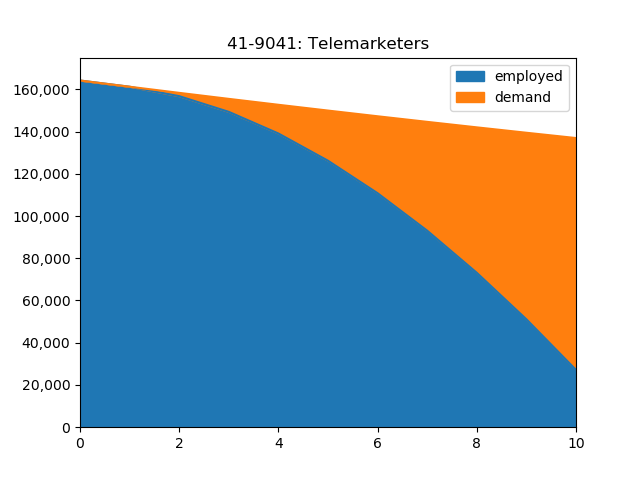
\includegraphics[scale=0.45]{Telemarketers.png}
    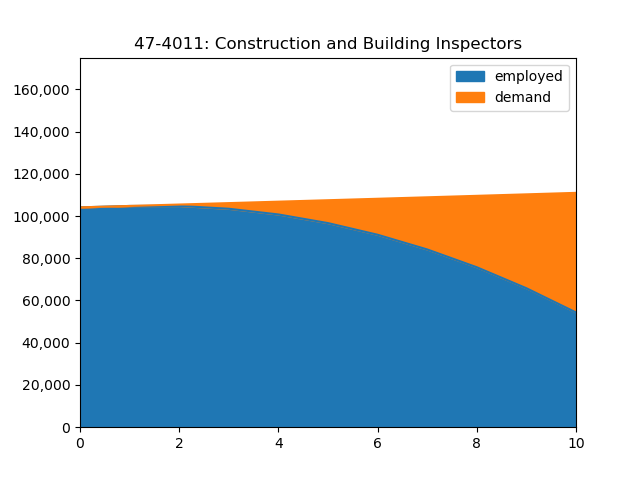
\includegraphics[scale=0.45]{Construction_and_Building_Inspectors.png}
    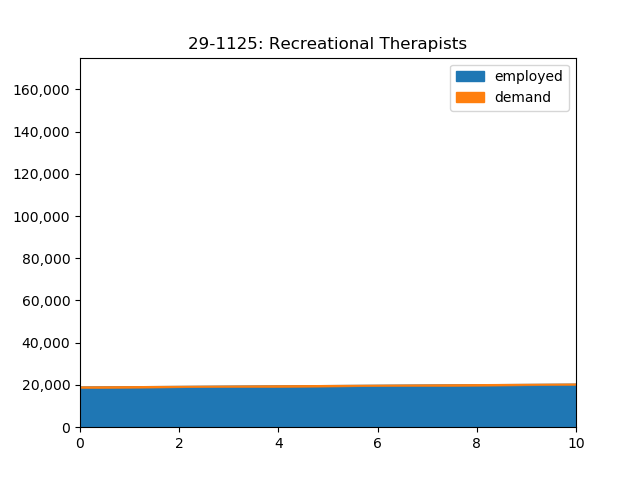
\includegraphics[scale=0.45]{Recreational_Therapists.png}
    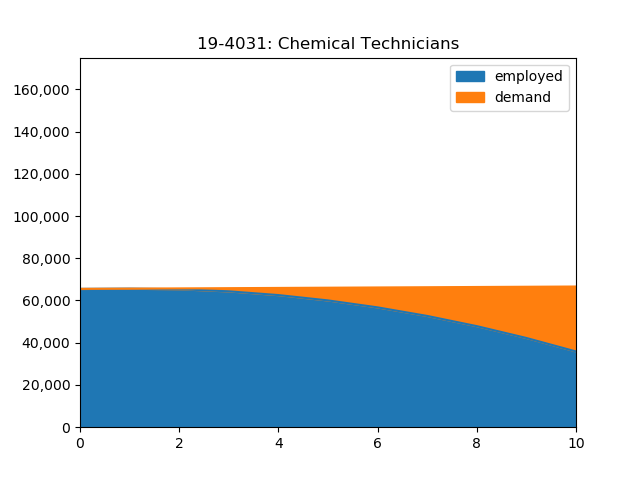
\includegraphics[scale=0.45]{Chemical_Technicians.png}
    \caption{10-year national employment loss against demand}
    \label{fig:graphs}
\end{figure}

\begin{table}[H]
\begin{threeparttable}
\caption{MSA-level job loss over most impacted State-level occupations}
\begin{tabular}{llllll}
MSA                                           & 39-9021\tnote{1} & 35-3021\tnote{2} & 41-2031\tnote{3} & 41-2011\tnote{4} & 53-7062\tnote{5} \\
\hline
Bakersfield, CA                               & 5,791    & 7,554    & 5,472    & 7,088    & 5,609    \\
Chico, CA                                     & 3,445    & 2,471    & 1,736    & 1,825    & 872      \\
El Centro, CA                                 & 3,151    & 1,109    & 2,259    & 1,668    & 462      \\
Fresno, CA                                    & 13,901   & 8,899    & 7,389    & 8,156    & 5,788    \\
Hanford-Corcoran, CA                          & 1,280    & 954      & 891      & 990      & 358      \\
Los Angeles-Long Beach-Anaheim, CA            & 188,484  & 132,977  & 118,982  & 115,502  & 110,112  \\
Madera, CA                                    & 1,494    & 858      & 708      & 1,047    & 536      \\
Merced, CA                                    & 2,237    & 1,648    & 2,091    & 1,846    & 903      \\
Modesto, CA                                   & 4,032    & 5,822    & 4,736    & 4,958    & 3,297    \\
Napa, CA                                      & 1,539    & 1,391    & 1,591    & 1,454    & 496      \\
Oxnard-Thousand Oaks-Ventura, CA              & 6,995    & 7,731    & 9,766    & 8,365    & 4,263    \\
Redding, CA                                   & 2,419    & 1,231    & 1,631    & 2,200    & 578      \\
Riverside-San Bernardino-Ontario, CA          & 43,504   & 42,161   & 36,802   & 36,895   & 60,791   \\
Sacramento--Roseville--Arden-Arcade, CA       & 28,065   & 22,586   & 20,127   & 18,595   & 19,988   \\
Salinas, CA                                   & 3,297    & 3,752    & 3,006    & 4,086    & 2,487    \\
San Diego-Carlsbad, CA                        & 25,516   & 34,145   & 30,650   & 30,031   & 17,040   \\
San Francisco-Oakland-Hayward, CA             & 58,468   & 45,302   & 36,287   & 40,052   & 26,012   \\
San Jose-Sunnyvale-Santa Clara, CA            & 18,321   & 18,402   & 16,011   & 15,918   & 11,139   \\
San Luis Obispo-Paso Robles-Arroyo Grande, CA & 3,454    & 3,344    & 3,998    & 2,341    & 1,047    \\
Santa Cruz-Watsonville, CA                    & 2,622    & 3,105    & 2,372    & 2,184    & 654      \\
Santa Maria-Santa Barbara, CA                 & 2,897    & 4,556    & 3,233    & 4,141    & 1,589    \\
Santa Rosa, CA                                & 5,249    & 4,312    & 4,715    & 4,511    & 2,713    \\
Stockton-Lodi, CA                             & 6,409    & 7,114    & 5,781    & 5,069    & 10,678   \\
Vallejo-Fairfield, CA                         & 4,641    & 3,490    & 3,681    & 3,913    & 2,395    \\
Visalia-Porterville, CA                       & 2,984    & 3,675    & 3,585    & 3,518    & 3,321    \\
Yuba City, CA                                 & 1,567    & 1,454    & 1,115    & 1,108    & 751      \\
\hline
Sum                                           & 441,762  & 370,043  & 328,615  & 327,461  & 293,879
\end{tabular}
\begin{tablenotes}
    \item[1] Personal Care Aides
    \item[2] Combined Food Preparation and Serving Workers, Including Fast Food
    \item[3] Retail Salespersons
    \item[4] Cashiers
    \item[5] Laborers and Freight, Stock, and Material Movers, Hand
\end{tablenotes}
\end{threeparttable}
\label{table:1}
\end{table}

\section{Conclusion}

This paper brings together real-time data sources and automation forecasts at a large scale in one simulated environment. The simulation produces an estimation of employment loss at the national and metropolitan state area levels. Outputs can be visualized at varying levels of granularity and the data cleaning, simulation, and graphing scripts are flexible and easily extendable. Further analysis of the simulation outputs reveals which communities face a high risk of job loss and can be used to inform policy decisions. A relatively straightforward extension of this work would be add policy scenarios to judge the impact of timing and intensity of training for new economy jobs making it a useful policy making tool. Further extensions of this work could include data sets from MSAs outside of California and build atop Frey and Osborne's work to create a truly real-time source of truth which can automatically pull new data sets from online sources, compute automation probabilities and clean data sets, and provide new 10-year job loss forecasts every year.

\bibliographystyle{plain}
\bibliography{final-paper}

\appendix

\section{Running the Programs}

There are 4 programs: \texttt{setup}, \texttt{cleanData}, \texttt{sim}, and \texttt{graph}. \texttt{setup} will create the required file structure (if it is not already present - see Appendix B). \texttt{cleanData} reads raw data files from \texttt{raw\_data\_files/}, cleans them, and saves them to \texttt{clean\_data\_files/} to be fed into the simulation. \texttt{sim} reads clean data files from \texttt{clean\_data\_files/}, runs the simulation using any options specified, and outputs the results of the simulation run into \texttt{sim\_outputs/}. \texttt{graph} reads the output files from \texttt{sim\_outputs/}, creates graphs based on the granularity options specified and displays/saves the graphs based on other specified options. Graphs are saved to \texttt{graphs/}.\\\\ To run any of the programs, navigate to the directory containing the programs in a new command line window. To run \texttt{setup}, simply type \texttt{./setup} in the terminal. To run any of the other programs, type \texttt{./<program\_name> -h} for a detailed help message on how to run. Examples are included below:
\begin{enumerate}
    \item \texttt{./sim -a} \\ This will run the simulation over the national data and all MSAs. MSA results will be written to \texttt{sim\_outputs/msa/} and national results will be written to \texttt{sim\_outputs/national\_output.xlsx}.
    \item \texttt{./cleanData --msa --clean-emp} \\ Clean and save all MSA employment data files to \texttt{clean\_data\_files/employment/msa}.
    \item \texttt{./graph --nat --soc 41-9041 47-4011 29-1125 19-4031 --ylim 170000} \\ This was the command used to generate the graphs shown in Figure 1. \texttt{--nat} tells the program to graph national-level data. \texttt{--soc} tells the program to generate individual graphs for the given SOCs, at the granularity levels specified (e.g. national or MSA). \texttt{--ylim} sets the y-axis limit for every graph created.
\end{enumerate}

\section{File Structure}
The programs read and write data that is organized in a specific structure. Running the \texttt{setup} command will produce this structure. While easily extendable, the file structure of the directory from which the programs are run must conform to the following:
\dirtree{%
    .1 /.
    .2 raw\_data\_files/.
    .3 projections/.
    .4 alltb6/.
    .3 employment/.
    .4 oesm18ma/.
    .4 oesm18nat/.
    .2 clean\_data\_files/.
    .3 projections/.
    .4 regional/.
    .4 msa/.
    .3 employment/.
    .4 msa/.
    .3 merged/.
    .4 msa/.
    .2 sim\_outputs/.
    .3 msa/.
    .2 graphs/.
    .3 msa/.
    .3 occupations/.
    .4 national/.
    .4 <MSA\_NAME>/.
}
\smallskip
"MSA\_NAME" is a substitute that represents a folder for every single MSA.


\end{document}
